\section{The Challenge}
	\subsection{Goals}
	\begin{frame}
		\frametitle{The Challenge}

		\begin{columns}
			\column[c]{.60\textwidth}
			
			\only<1>{
		    \begin{itemize}
			    \item 12th May 2014 - \\15th September 2014
			    \item 13,000\$ prize money
			    \item 1,943 participants \\in 1,785 teams
		    \end{itemize}
		    }
		    \only<2>{
		    \frametitle{The Challenge - Goals}
		    \begin{block}{Promote data science in physics}			   
	      		\begin{quote}
		    		"The Higgs boson machine learning challenge [...] has been 
		    		set up to promote collaboration between high energy 
		    		physicists and data scientists."
				    \cite{higgsPaper}
			    \end{quote}
   			\end{block}
		    }
		 	
		    \only<3>{
		    \frametitle{The Challenge - Goals}
		    \begin{block}{Improve classification}			    
	      		\begin{quote}
		    		"We expect that significant improvements are possible by 
		    		re-visiting some of the ad hoc choices in the standard 
		    		procedure [...]."
				    \cite{higgsPaper}
			    \end{quote}
   			\end{block}
		    }
		    
		    \only<4>{
		    \frametitle{The Challenge - Goals}
		    \begin{block}{Strengthen the discovery}			    
	      		\begin{quote}
		    		"The goal of the Higgs Boson Machine Learning Challenge is 
		    		[...] to improve the discovery significance of the 
		    		experiment."
				    \cite{higgsChallenge}
			    \end{quote}
   			\end{block}
		    }
		    \column[c]{.50\textwidth}
		    
\includegraphics[width=130pt]{images/higgs_logo}
		\end{columns}		
		
	\end{frame}
	
	\subsection{Data}
	\begin{frame}
		\frametitle{The Challenge - Data}
		
		Provided Data is simulated in a two-step procedure.\\
		Technical properties of ATLAS are actually visible in some features.
		
		\begin{columns}			
			\column[c]{.50\textwidth}
				\begin{figure}
					\centering
					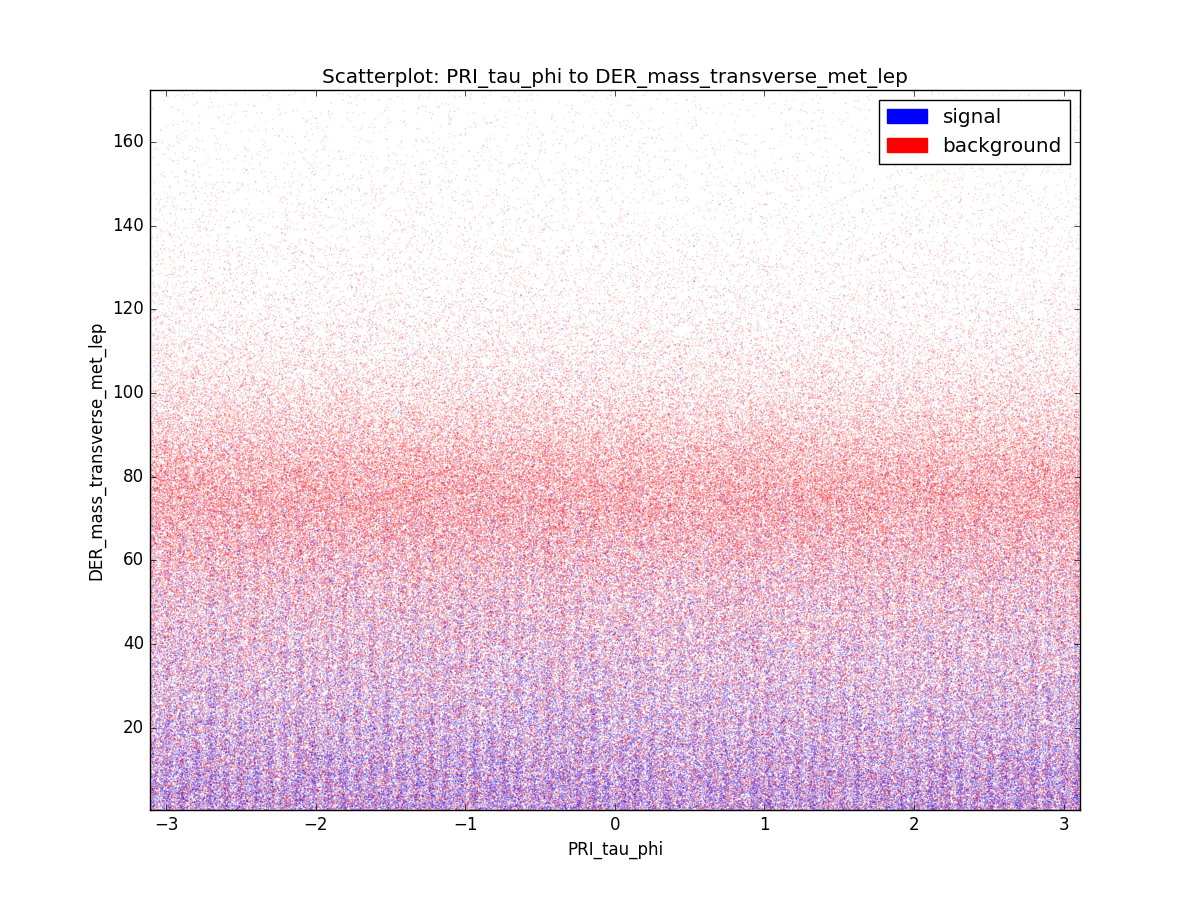
\includegraphics[width=130pt]{images/PRI_tau_phi}
					\caption{Scatterplot of PRI\_tau\_phi to a feature 
							 beneficial for demonstration}
				\end{figure}
								
			\column[c]{.50\textwidth}
				\begin{figure}
					\centering
					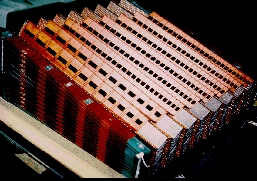
\includegraphics[width=130pt]{images/calo}
					\caption{Inner sections of the calorimeter in ATLAS
						\cite{ATLASpage}}
				\end{figure}
		\end{columns}			

	\end{frame}
		
	\begin{frame}
		\frametitle{The Challenge - Data}
		\begin{itemize}
			\item Five features with challenge-relevant information\\
				  (only needed for submission and its evaluation)
			\item 30 features with simulated data \\
				  (classification-relevant)
			\item simulated data has dimension $ dim(data)=800000*30 $
			
		\end{itemize}
	\end{frame}
		
		
	\subsection{Evaluation}
	\begin{frame}
		\frametitle{The Challenge - Evaluation}
			
		\begin{block}{Approximate Median Significance (AMS)}
			$$AMS = \sqrt{2 { (s + b + b_r) log[1 + (s/(b+b_{r}))] - s}} $$
			where: \begin{itemize}
				\item $ b_{r} = 10 $ is a regulization term (set by the 
					contest),
				\item $ b = \sum_{i=1}^{n} w_i, y_i=0 $ is sum of weighted
					background (incorrectly classified as signal),
				\item $ s = \sum_{i=1}^{n} w_i, y_i=1 $ is sum of weighted 
					signals (correctly classified as signal),
				\item $ log $ is natural logarithm
			\end{itemize}
		\end{block}			
	\end{frame}
	
	\subsection{Task}
	\begin{frame}
		\frametitle{The Challenge - Task}
		\begin{enumerate}
			\item learn connection between data and signal-/background-likelihood
			\item classify the test-data (550,000 events)
			\item submit in format\\
				  $EventId,RankOrder,Class$\\
				  $1,2,b$\\
  				  $2,541234,s$\\
  				  \ldots
		\end{enumerate}
	\end{frame}